%!TEX program = xelatex

\documentclass[a4paper, openany, oneside]{memoir}
\usepackage[no-math]{fontspec}
\usepackage{pgfplots}
\pgfplotsset{compat=newest}
\usepackage{commath}
\usepackage{mathtools}
\usepackage{amssymb}
\usepackage{amsthm}
\usepackage{booktabs}
\usepackage{mathtools}
\usepackage{xcolor}
\usepackage[separate-uncertainty=true, per-mode=symbol]{siunitx}
\usepackage[noabbrev, capitalize]{cleveref}
\usepackage{listings}
\usepackage[american inductor, european resistor]{circuitikz}
\usepackage{amsmath}
\usepackage{amsfonts}
\usepackage{ifxetex}
\usepackage[dutch,english]{babel}
\usepackage[backend=bibtexu,texencoding=utf8,bibencoding=utf8,style=ieee,sortlocale=en_GB,language=auto]{biblatex}
\usepackage[strict,autostyle]{csquotes}
\usepackage{parskip}
\usepackage{import}
\usepackage{standalone}
\usepackage{hyperref}
%\usepackage[toc,title,titletoc]{appendix}

\ifxetex{} % Fonts laden in het geval dat je met Xetex compiled
    \usepackage{fontspec}
    \defaultfontfeatures{Ligatures=TeX} % To support LaTeX quoting style
    \setromanfont{Palatino Linotype} % Tover ergens in Font mapje in root.
    \setmonofont{Source Code Pro}
\else % Terug val in standaard pdflatex tool chain. Geen ondersteuning voor OTT fonts
    \usepackage[T1]{fontenc}
    \usepackage[utf8]{inputenc}
\fi
\newcommand{\references}[1]{\begin{flushright}{#1}\end{flushright}}
\renewcommand{\vec}[1]{\boldsymbol{\mathbf{#1}}}
\newcommand{\uvec}[1]{\boldsymbol{\hat{\vec{#1}}}}
\newcommand{\mat}[1]{\boldsymbol{\mathbf{#1}}}
\newcommand{\fasor}[1]{\boldsymbol{\tilde{\vec{#1}}}}
\newcommand{\cmplx}[0]{\mathrm{j}}
\renewcommand{\Re}[0]{\operatorname{Re}}
\newcommand{\Cov}{\operatorname{Cov}}
\newcommand{\Var}{\operatorname{Var}}
\newcommand{\proj}{\operatorname{proj}}
\newcommand{\Perp}{\operatorname{perp}}
\newcommand{\col}{\operatorname{col}}
\newcommand{\rect}{\operatorname{rect}}
\newcommand{\sinc}{\operatorname{sinc}}
\newcommand{\IT}{\operatorname{IT}}
\newcommand{\F}{\mathcal{F}}

\newtheorem{definition}{Definition}
\newtheorem{theorem}{Theorem}


\DeclareSIUnit{\voltampere}{VA} %apparent power
\DeclareSIUnit{\pii}{\ensuremath{\pi}}

\hypersetup{%setup hyperlinks
    colorlinks,
    citecolor=black,
    filecolor=black,
    linkcolor=black,
    urlcolor=black
}

% Example boxes
\usepackage{fancybox}
\usepackage{framed}
\usepackage{adjustbox}
\newenvironment{simpages}%
{\AtBeginEnvironment{itemize}{\parskip=0pt\parsep=0pt\partopsep=0pt}
\def\FrameCommand{\fboxsep=.5\FrameSep\shadowbox}\MakeFramed{\FrameRestore}}%
{\endMakeFramed}

% Impulse train
\DeclareFontFamily{U}{wncy}{}
\DeclareFontShape{U}{wncy}{m}{n}{<->wncyr10}{}
\DeclareSymbolFont{mcy}{U}{wncy}{m}{n}
\DeclareMathSymbol{\Sha}{\mathord}{mcy}{"58}
\addbibresource{../../../../includes/bibliography.bib}

\begin{document}


\section{Reconstruction of the power spectral density}
\label{sec:reconstruction-algorithm}
This section will discuss an algorithm to estimate in real-time the power spectral density of a signal which is sampled at sub-Nyquist frequencies. We consider multi-coset sampling such as described in \cref{cha:sampling}. A step-by-step derivation of the algorithm can be found in \cref{sec:reconstruction-derivation}.

\subsection{Reconstruction and multi-coset sampling}
Let the input signal sampled at the Nyquist frequency be denoted by $x[n]$. Let the number of cosets be given by $M$. Let the output of coset $i$ be denoted by $y_i[n]$. Our reconstruction method estimates the power spectral density of $x[n]$ by making use of the outputs of all cosets. The Wiener-Khinchin theorem shows that estimating the power spectral density of $x[n]$ is equivalent to estimating the autocorrelation of $x[n]$.\footnote{More specifically, the Wiener-Khinchin theorem states that the Fourier transform of the autocorrelation equals the power spectral density, which yields the equivalence.} Therefore, our reconstruction method aims to estimate the autocorrelation of $x[n]$. Let the autocorrelation of the input signal be denoted by $r_x[m]$. Let the cross-correlation of the output of cosets $i$ and $j$ be denoted by $r_{y_i,y_j}[m]$. We will make use of $r_{y_i,y_j}[m]$ to estimate $r_x[m]$. This estimation is based on the relationship
\begin{align*}
    \vec{r}_{y} = \mat{R} \vec{r}_x.
\end{align*}
Here $\vec{r}_y$ represents an aggregation of $r_{y_i,y_j}[m]$ and $\vec{r}_x$ represents an aggregation of $r_x$. We see that we can use $\mat{R}$ to relate $r_x[m]$ to $r_{y_i,y_j}[m]$. So $\mat{R}$ represents the relationship between the autocorrelation of the input signal and the cross-correlations of the outputs of the cosets.

Before we describe the algorithm, we have to study the output of a coset more closely. Every coset $i$ is associated to a sampling signal $c_i[n]$. \textbf{Also, every coset samples the input signal such that it consists of every $N$'th sample of $x[n]$. However, which $N$'th sample may differ between the cosets.} Therefore, if we divide the input signal in groups of $N$ samples, then the output of a coset consists of the same sample of every group of $N$ samples. This concept is illustrated in \cref{fig:illustration-yi}. The sampling signal of coset $i$ is such that $c_i[n]=1$ if coset $i$ samples the $N-n$'th sample of every group of $N$ samples of the input signal. This concept is discussed carefully in \cref{sec:reconstruction-derivation}. Also, this concept will be discussed in \cref{cha:sampling_methods}.

\subsection{Algorithm}
It is clear that $y_i[n]$ is part of the input of the algorithm. The way all cosets sample the input signal, however, is determined by the sampling technique. The configuration refers to the way all cosets sample the input signal. Possible configurations are discussed in \cref{cha:sampling} and will be further discussed in \cref{cha:sampling_methods}. Furthermore, the input of the algorithm also consists of the parameters $M$, $N$, $L$ and $K$. Here $M$ and $N$ have already been discussed. The parameter $L$ limits $r_{y_i,y_j}[m]$ in support from $m=-L$ to $m=L$.\footnote{If $r_{y_i,y_j}[m]$ is limited in support from $m=-L$ to $m=L$, then this means that $r_{y_i,y_j}[m]=0$ for $|m|>L$.} This influences the length of the estimated autocorrelation, which then determines the resolution of the estimated power spectral density of $x[n]$. The autocorrelation $r_x[m]$ will be estimated for $|m| \le LN$. The parameter $K$ influences the measurement time, which determines the accuracy of the estimated power spectral density. The measurement time consists of the time required to obtain $KL$ samples of the output of every coset. The inputs and output of the algorithm are summarised in Table \ref{tab:reconstruction-algorithm-inputs-outputs}.


\begin{figure}
\centering
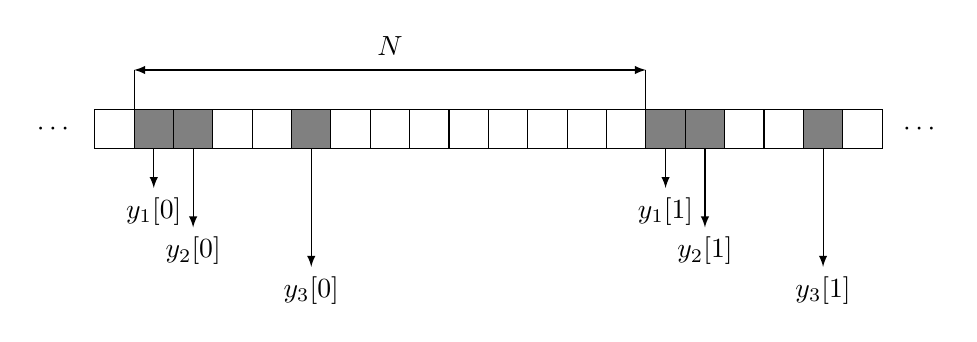
\begin{tikzpicture}
\draw  (-1,-4) rectangle (-0.5,-4.5);
\draw  [fill=gray](-0.5,-4) rectangle (0,-4.5);
\draw  [fill=gray](0,-4) rectangle (0.5,-4.5);
\draw  (0.5,-4) rectangle (1,-4.5);
\draw  (1,-4) rectangle (1.5,-4.5);
\draw  [fill=gray](1.5,-4) rectangle (2,-4.5);
\draw  (2,-4) rectangle (2.5,-4.5);
\draw  (2.5,-4) rectangle (3,-4.5);
\draw  (3,-4) rectangle (3.5,-4.5);
\draw  (3.5,-4) rectangle (4,-4.5);
\draw  (4,-4) rectangle (4.5,-4.5);
\draw  (4.5,-4) rectangle (5,-4.5);
\draw  (5,-4) rectangle (5.5,-4.5);
\draw  (5.5,-4) rectangle (6,-4.5);
\draw  [fill=gray](6,-4) rectangle (6.5,-4.5);
\draw  [fill=gray](6.5,-4) rectangle (7,-4.5);
\draw  (7,-4) rectangle (7.5,-4.5);
\draw  (7.5,-4) rectangle (8,-4.5);
\draw  [fill=gray](8,-4) rectangle (8.5,-4.5);
\draw  (8.5,-4) rectangle (9,-4.5);
\draw (-0.5,-4) -- (-0.5,-3.5);
\draw (6,-4) -- (6,-3.5);
\draw [>=latex,<->] (-0.5,-3.5) -- node[yshift=0.3cm] {$N$} (6,-3.5);
\draw [>=latex,->] (-0.25,-4.5) -- node[pos=1, yshift=-0.3cm] {$y_1[0]$} (-0.25,-5);
\draw [>=latex,->] (-0.25+6.5,-4.5) -- node[pos=1, yshift=-0.3cm] {$y_1[1]$} (-0.25+6.5,-5);
\draw (-1.5,-4.25) node {$\cdots$};
\draw (9.5,-4.25) node {$\cdots$};
\draw [>=latex,->] (-0.25+0.5,-4.5) -- node[pos=1, yshift=-0.3cm] {$y_2[0]$} (-0.25+0.5,-5.5);
\draw [>=latex,->] (-0.25+6.5+0.5,-4.5) -- node[pos=1, yshift=-0.3cm] {$y_2[1]$} (-0.25+6.5+0.5,-5.5);
\draw [>=latex,->] (-0.25+2,-4.5) -- node[pos=1, yshift=-0.3cm] {$y_3[0]$} (-0.25+2,-6);
\draw [>=latex,->] (-0.25+6.5+2,-4.5) -- node[pos=1, yshift=-0.3cm] {$y_3[1]$} (-0.25+6.5+2,-6);
\end{tikzpicture}
\caption{Illustration of how $y_i[n]$ is constructed from $x[n]$. The blocks represent the samples of $x[n]$.}
\label{fig:illustration-yi}
\end{figure}

The algorithm consists of following steps.

\begin{table}
    \centering
    \begin{tabularx}{\textwidth}{llY}
        \textbf{Type} & \textbf{Parameter} & \textbf{Description} \\ \hline
        Input & $M$ & Number of cosets \\
        Input & $N$ & Downsampling factor. Every coset samples the input signal once per $N$ samples. \\
        Input & $y_i[n]$ & Output of coset $i$ \\
        Input & $L$ & Support of $r_{y_i,y_j}[m]$. This parameter influences the resolution of the estimated power spectral density of $x[n]$. \\
        Input & $K$ & Oversampling factor. This parameter influences the accuracy of the estimated power spectral density of $x[n]$, but increases the measurement time. The measurement time consists of the time required to obtain $KL$ samples of the output of every coset. \\
        Output & $r_x[m]$ & Autocorrelation of $x[n]$. The autocorrelation $r_x[m]$ is estimated for $|m| \le LN$.
    \end{tabularx}
    \caption{Input and outputs of the reconstruction algorithm}
    \label{tab:reconstruction-algorithm-inputs-outputs}
\end{table}

\begin{enumerate}[labelindent=0pt,labelwidth=\widthof{\ref{last-item1}},label=Step \arabic*:,itemindent=1em,leftmargin=!]
    \item Determine $c_i[n]$ for every coset $i$. \\
    The configuration determines $c_i[n]$ for every coset $i$. How $c_i[n]$ can be obtained from the configuration is explained in \cref{cha:sampling_methods}. The restrictions on $c_i[n]$ are discussed in \cref{sub:reconstruction-ci}.
    \item Construct $\mat{R}$. \\
    \cref{sub:reconstruction-generation} explains how to construct $\mat{R}$.
    \item Measure $y_i[n]$ for $KL$ samples for every coset $i$.
    \item Estimate $r_{y_i,y_j}[m]$ for every combination of cosets $i$ and $j$. \\
    \cref{sub:reconstruction-estimation} discusses how $KL$ samples of $y_i[n]$ can be used to estimate $r_{y_i,y_j}[m]$.
    \item Construct $\vec{r}_y$. \\
    If
    \begin{align*}
        \vec{r}_{y_i,y_j} = \begin{bmatrix}
            r_{y_i,y_j}[L] \; \cdots \; r_{y_i,y_j}[-L]
        \end{bmatrix},
    \end{align*}
    then
    \begin{align*}
        \vec{r}_y = \begin{bmatrix}
            \vec{r}_{y_1,y_1} \\ \vdots \\ \vec{r}_{y_M,y_M}
        \end{bmatrix}^T.
    \end{align*}
    \item Calculate $\vec{r}_x=\mat{R}^\dagger \vec{r}_y$, which yields an estimation of $r_x[m]$. \\
    Here
    \begin{align*}
         \vec{r}_x = \begin{bmatrix}
             r_x[LN] \; \cdots \; r_x[-LN]
         \end{bmatrix}.
    \end{align*} This means that the autocorrelation $r_x[m]$ is estimated for $|m| \le LN$, as stated earlier. The matrix $\mat{R}^\dagger$ denotes the Moore-Penrose pseudoinverse of $\mat{R}$.
    \label{last-item1}
\end{enumerate}

\end{document}